\documentclass[12pt,twoside]{article}
\usepackage{amsmath}
\usepackage{graphicx}
\usepackage{hyperref}
\title{EDFM V1.0}
\author{Luca Formaggia, Luca Turconi, Anna Scotti\\MOX, Politecnico di Milano}
\date{July 2013}
\begin{document}
\maketitle
\section{Introduction}
EDFM is a program for computing geometry related quantities to determine the transmission factors in a corner point grid cutted by a fracture network.

It reads two sets of files, one related to the corner point grid, and a file containing the description of the fractures.
The definition of where the files are stored and some additional parameter are read form a \texttt{GetPot} file. For more information about a GetPot file
you may consult \href{getpot.sourceforge.net}{getpot.sourceforge.net}

The file is called by default \texttt{data.pot}, but the name may be changed using the option \texttt{InputFile=string} when launching the program:

\begin{verbatim}
main_edfm InputFile=myfile.pot
\end{verbatim}

\subsection{The GetPot file}
We give a brief description of the file 
\begin{verbatim}
GridFile=./data/GRID_FINE_no_map.GRDECL #name of corner point grid file
FractureFile=./data/lista_mia2.fab #name of file with fractures
conv_z=1   #=1 if z coordinates of grid and fracture is coherent
           #=-1 otherwise 
isOPT=yes  #TO use optimized method

#----------- distorsion of grid and fractures 
#            (normally deactivated)
theta_x=0  #grid distortion angle (degree)
theta_y=0  #grid distortion angle (degree)
direzione=x #direction of applied shear

theta_xF=0  #fracture distortion angle (degree)
theta_yF=0  #fracture distortion angle (degree)
direzioneF=x #direction of applied shear

rotate_z=no  #rotate grid around z axis to align edges with x,y

#Output section

exportFractures=yes # export the fractures (bilinear patches) for visualization with paraview
exportFrGrids=yes   # export the grids of the fractures resulting from the intersection with the cells for visualization with Paraview
exportGeoprop=yes   # export volumes, intersection areas and mean distance of the cut cells for visualization with Paraview
exportIntersections=yes #  export the insersection points for visualization with Paraview
exportGrid=yes # export the corner point grid for visualization with Paraview
outpath=./output #Output file directory
\end{verbatim}
The output files are stored in the directory indicated in the file, Note that \emph{if the directory is
not existent or if \texttt{outpath} is not set (or set to the empty string), no output file will be generated}
\section{Files}
\subsection{Corner point grid file}
A corner point grid is a grid where the basic element is a cell with 6 faces (logically a cube) and  which is defined through vertical pillars 
on a two dimensional horizontal map. A cell is then identified by three indexes $i,j,k$.

\begin{figure}
	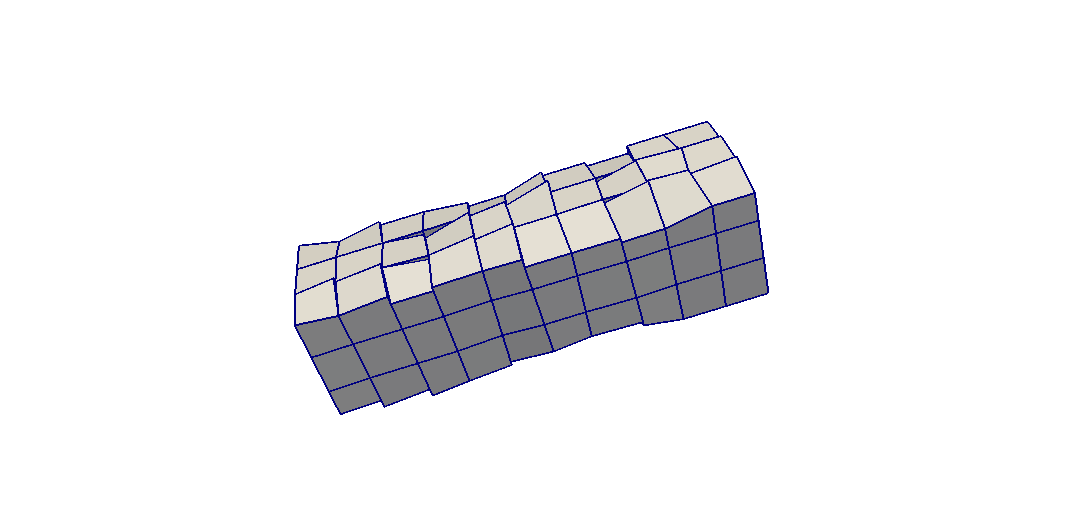
\includegraphics[scale=0.3]{./img/CPgrid.png}
	\caption{Example of corner point grid}
\end{figure}

The code accepts in input corner points grids in the ASCII format used by the
ECLIPSE software by Schlumberger. 

Also the fracture file is the standard ASCII file used by ????? 

\subsection{Output file}
The output produces $N_F$ files, where $N_F$ 
is the number of fractures. For each fracture we produce an ASCII file called
 \emph{fratturaN.txt}, of which we give an example
\begin{verbatim}
FRACTURE 1
Ne  72
Nf	Ncella	i	j	k	PV		AREA		DMEAN		TMF
1	1	(5	18	8)	17.3532		1735.32		61.408		0.240963
...

NN connections Horizontal
NF	Nc	i	j	k	---------	NF	Nc	i	j	k		 T

1	1	(5	18	8)	---------	1	2	(5	17	8)		11.3924
...
--------------------------------------------------------

NN connections Vertical
NF	Nc	i	j	k	---------	NF	Nc	i	j	k		 T

1	1	(5	18	8)	---------	1	10	(5	18	9)		1037.89
...

--------------------------------------------------------
Intersections 
WITH	2
Nf1	Nc1	---------	Nf2	Nc2		dmedio	Tf1f2
1	4	---------	2	6		96.7366	5.68371
...
\end{verbatim}

We report the number of cells intersected by the fracture, $N_e$, which correspond to the number of fracture cells generated. 
They are ordered following the increasing $y$ coordinate of the centroid. 
In the case of equal $y$ coordinates, the ordering follows the increasing $x$ coordinates.
For each cell we have:
\begin{itemize}
 \item The fracture number
 \item The cell number
 \item The corresponding ijk coordinates
 \item The pore volume
 \item The area
 \item The average cell-fracture distance
 \item The computer fracture-matrix trasmissibility
\end{itemize}

Then, it is reported the trasmissibility between fracture elements, subdivided into horizontal and vertical.
Then we have the coordinates of the two adjacent cells, followed by the value of the corresponding trasmissibility.
Finally, we consider the intersection with other fractures. After the keyword
\textbf{Intersections} we report which other fracture is intersected, and in which cell, by reporting the numbering of the fractured cells, with the corresponding trasmissibility.

Beside these information, it is possible to export some useful files for the visualization with \emph{ParaView}. In particular we hace a file by which it is possible to chow the fracture geometry with the grids generated by the intersections, the intersection points and quantities like the intersection areas or the average distance fracture/cell center.
\end{document}


%%% Local Variables: 
%%% mode: latex
%%% TeX-master: t
%%% End: 
